\Chapter{Tervezés}

\Section{Felhasznált technológiák}

\SubSection{C\#}

Az egyetemi éveim alatt lehetőségem volt 2 féléven keresztül az evosoft Hungary Kft. evoCampus-án részt venni, ahol megismerkedtem a C\# nyelvvel, amelyet végül az alkalmazásom megvalósításához választottam.

A C\# egy általános célú, objektumorientált programozási nyelv, valamint a .NET környezet egyik fő programozási nyelve. A C nyelvcsaládhoz tartozik, így ismert lehet a C++ és Java programozók számára, hiszen ilyen alapokon fejlesztették ki. Platformfüggetlenségét a .NET környezet átvihetősége biztosítja.

A .NET keretrendszer gyors és hatékony alkalmazásfejlesztést biztosít a .NET osztálykönyvtárak által. A különböző nyelveken írt komponensek együttműködését pedig a CLR (\textit{Common Language Runtime}) és a CTS (\textit{Common Type Sytem}) segítségével könnyíti meg \cite{csharp}.

\SubSection{Visual Studio}

A Visual Studio egy integrált fejlesztői környezet, amelyet a Microsoft fejlesztett ki különböző alkalmazások, pl.: konzol, webalkalmazások, mobilalkalmazások fejlesztésére. Lehetőséget nyújt a C\#-on kívül például Viusal Basic, F\# és számos más nyelveken történő programozásra. Az alkalmazásom megvalósításakor én a \textit{Community} kiadást választottam, ami egy olyan ingyenes verzió, amely a \textit{Professional} kiadáshoz hasonló szolgáltatásokat tartalmaz \cite{vs}.

\SubSection{WPF}

A WPF (\textit{Windows Presentation Foundation}) egy grafikus felhasználói felületet biztosító keretrendszer. Előnye a XAML nyelv, amely megkönnyíti a felhasználói felület létrehozását és szerkesztését, valamint lehetővé teszi magának a UI tervezésének elkülönítését a program többi részétől. Emellett, lehetőség van adatkötés (\textit{DataBinding}) használatára, amely állandó kapcsolatot biztosít az alkalmazás felhasználói felülete és backend-en tárolt adatok között. Így, egy adat backend-en történő értékének megváltozása során a felhasználói felület automatikusan fog frissülni és fordítva \cite{wpf}, \cite{databinding}.

\SubSection{MahApps}

A \textit{MahApps} egy olyan keretrendszer, amely egy modernebb felhasználói felület elérését segíti a WPF-en keresztül \cite{mahapps}. Az alkalmazásom megvalósítása kezdetén kezdtem használni, viszont a későbbiekben háttérbe került a diagram \textit{Canvas}-sal történő fejlesztése miatt.

\SubSection{MVVM}

Az MVVM rövidítés a \textit{Model}, \textit{View}, \textit{ViewModel} szavakból származik. A séma lényege, hogy az alkalmazásunkat erre a három, jól elkülöníthető logikai egységre bontjuk szét, mely által jobban átláthatóvá válik (\ref{fig:mvvm}. ábra). A három egység különböző célokat szolgál.

\begin{figure}[h]
	\centering
	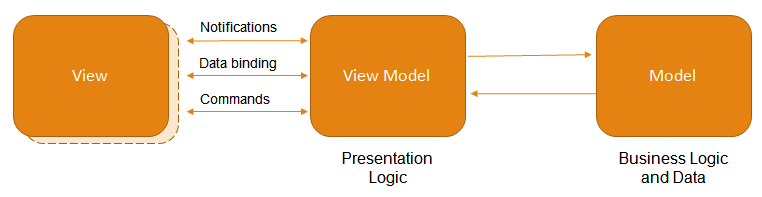
\includegraphics[scale=0.5]{images/mvvm.png}
	\caption{Az MVVM működése (forrás: \url{https://docs.devexpress.com/WPF/15112/mvvm-framework})}
	\label{fig:mvvm}
\end{figure}

A \textit{View} szerepe a grafikus felület biztosítása, minden, amit a képernyőn meg szeretnénk jeleníteni, azt megadhatjuk itt a XAML kód által. A XAML kódon belül definiáljuk a binding-okat is.

A \textit{Model} tartalmazza a különböző adatokat és osztályokat, amikkel dolgozni szeretnénk.

A \textit{ViewModel} pedig a kettő közötti kapcsolatot adja meg. Itt történik például a példányosítás, és ezáltal jeleníthetjük meg azt, amit a \textit{View}-n látni szeretnénk, általában \textit{command}-okon keresztül \cite{mvvm}.

\SubSection{Azure DevOps}

Az Azure DevOps (korábban \textit{Visual Studio Team Foundation Server}, röviden TFS) szoftverfejlesztői szolgáltatásokat nyújt csapatok számára az alkalmazások készítéséhez és a projektmunka hatékony végzéséhez. Személy szerint a verziókövetés (\ref{fig:azureHistory}. ábra) miatt tartottam fontosnak a használatát, mivel lehetővé teszi, hogy a kódban történő változtatásokat nyomon követhessem, engedélyezi, hogy szükség esetén egy korábbi változatra visszaálljak és nyilvántartja a különbségeket a verziók között. Különböző verziókat is összeilleszthetünk, ilyenkor a módosítások miatt felmerülő problémák esetén pedig a konfliktusok lekezelésére is lehetőség van \cite{azure}.

\begin{figure}[h]
	\centering
	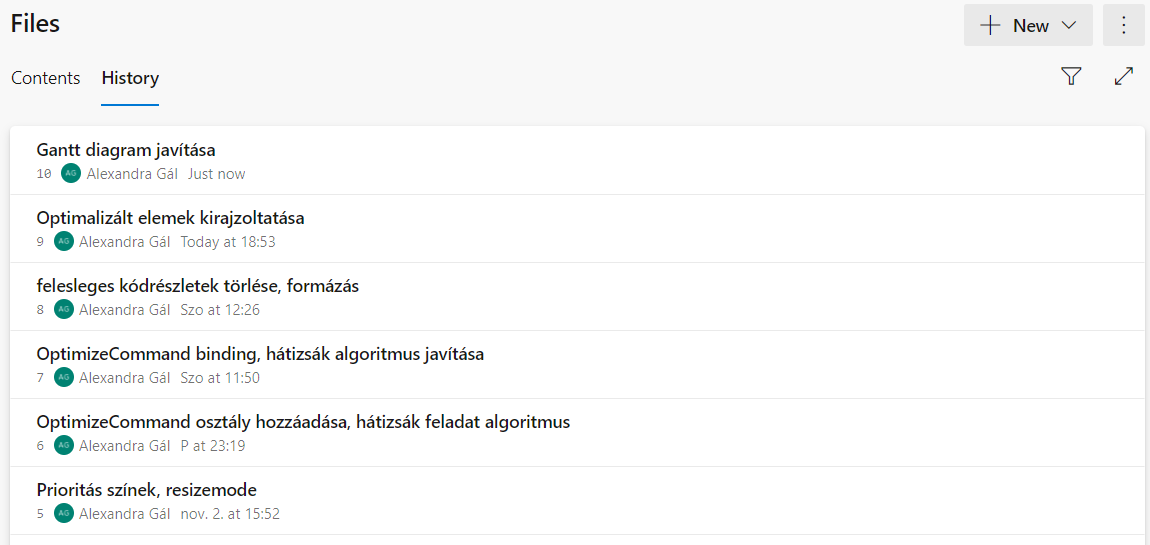
\includegraphics[scale=0.5]{images/azureHistory.png}
	\caption{Verziókövetés az Azure DevOps-ban}
	\label{fig:azureHistory}
\end{figure}

\SubSection{\texttt{ItemsControl}, \texttt{Canvas}, \texttt{Rectangle} osztályok}

Mivel C\#-ban a legtöbb lehetőség a diagramokat illetően a \textit{WinForms}-hoz kapcsolódik és nem a WPF-hez, vagy pedig nem nyílt forráskódú könyvtárak által lenne lehetséges, ezért úgy döntöttem, hogy a vizuális ábrázolást az \texttt{ItemsControl}, a \texttt{Canvas}, és a \texttt{Shape} könyvtár közül a \texttt{Rectangle} osztály segítségével oldom meg.
\begin{itemize}
	\item A \texttt{Rectangle} osztály segít a téglalapok megrajzolásában, ami a feladatok hosszát reprezentáló sávot ábrázolja majd a diagramon.
	\item A \texttt{Canvas} egy olyan területet biztosít, ahol elemeket tudunk pozícionálni.
	\item Az \texttt{ItemsControl} fogja tartalmazni a \texttt{Canvas}-t, amelyet az \texttt{ItemsControl} \\ \texttt{ItemsPanel}-jére tudunk elhelyezni.
\end{itemize}
Az \texttt{ItemsControl}-ra azért van szükség, mert a kirajzolandó téglalapok egy \texttt{Rectangle} típusú \texttt{ObservableCollection}-ben lesznek eltárolva és ez a \texttt{Control} a kollekciók elemeinek megjelenítését segíti.

\Section{UML diagram}

Az alkalmazás UML diagramja \aref{fig:uml}. ábrán látható. A program során az MVVM és \textit{Binding} használatát a \textit{Command}-ok segítik. A \textit{Command} osztályok kapcsolatban állnak a \textit{ViewModel}-lel, ami kapcsolatot létesít a UI felület és backend adatok között. Az \texttt{AddTaskCommand}-ban valósul meg a feladatok példányosítása, majd ezeknek a grafikus felületen történő megjelenítése a \texttt{DrawChart} osztályon belüli \texttt{DrawTasks} metódus által történik. Az \texttt{OptimizeCommand} osztály szolgál a feladatok ütemezésének és optimalizálásának végrehajtásához. A sorrendkialakítás a \texttt{KnapSack} osztály \texttt{OrderTasks} metódusa által, míg az ütemezési probléma megoldására választott hátizsák algoritmus a \texttt{KnapSackAlgorithm} metódus által valósul meg. A végső, kialakult ütemtervet a \texttt{DrawChart} osztályon belül a \texttt{DrawScheduledTasks} metódus által jeleníti meg az alkalmazás.

Az MVVM-es megközelítés miatt a \textit{Command}-okban szerepel egy-egy \texttt{CanExecute} metódus, amelyek után, \texttt{true} visszatérési érték esetén lefutnak az \texttt{Execute} metódusok, amelyek a végrehajtandó programkódokat -- mint például egy feladat példányosítása vagy az \texttt{OrderTasks} metódus meghívása -- tartalmazzák. A  \texttt{MainViewModel} által tartalmazott \texttt{RaisePropertyChanged} metódus szintén az MVVM fontos részeként szokott szerepelni, az \texttt{INotifyPropertyChanged} interfészhez és a \texttt{NotifyPropertyChanged} eseményhez kapcsolódva, amely a felhasználói felület felé történő változások értesítéséért és frissítésekért felel.
\begin{figure}[h]
	\centering
	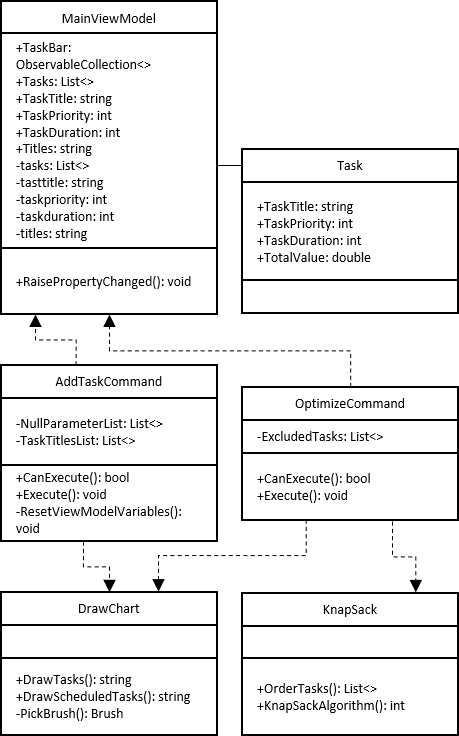
\includegraphics[scale=0.9]{images/uml.png}
	\caption{Az alkalmazás UML diagramja}
	\label{fig:uml}
\end{figure}
